% Capa, folha de rosto e verso da folha de rosto (versão PDF)
\usepackage{tikz}
\usepackage{graphicx}
\renewcommand{\maketitle}{%
  % Capa
  \begin{titlepage}
    \thispagestyle{empty}
    \begin{tikzpicture}[remember picture, overlay]
      \node[inner sep=0pt] at (current page.center)
        {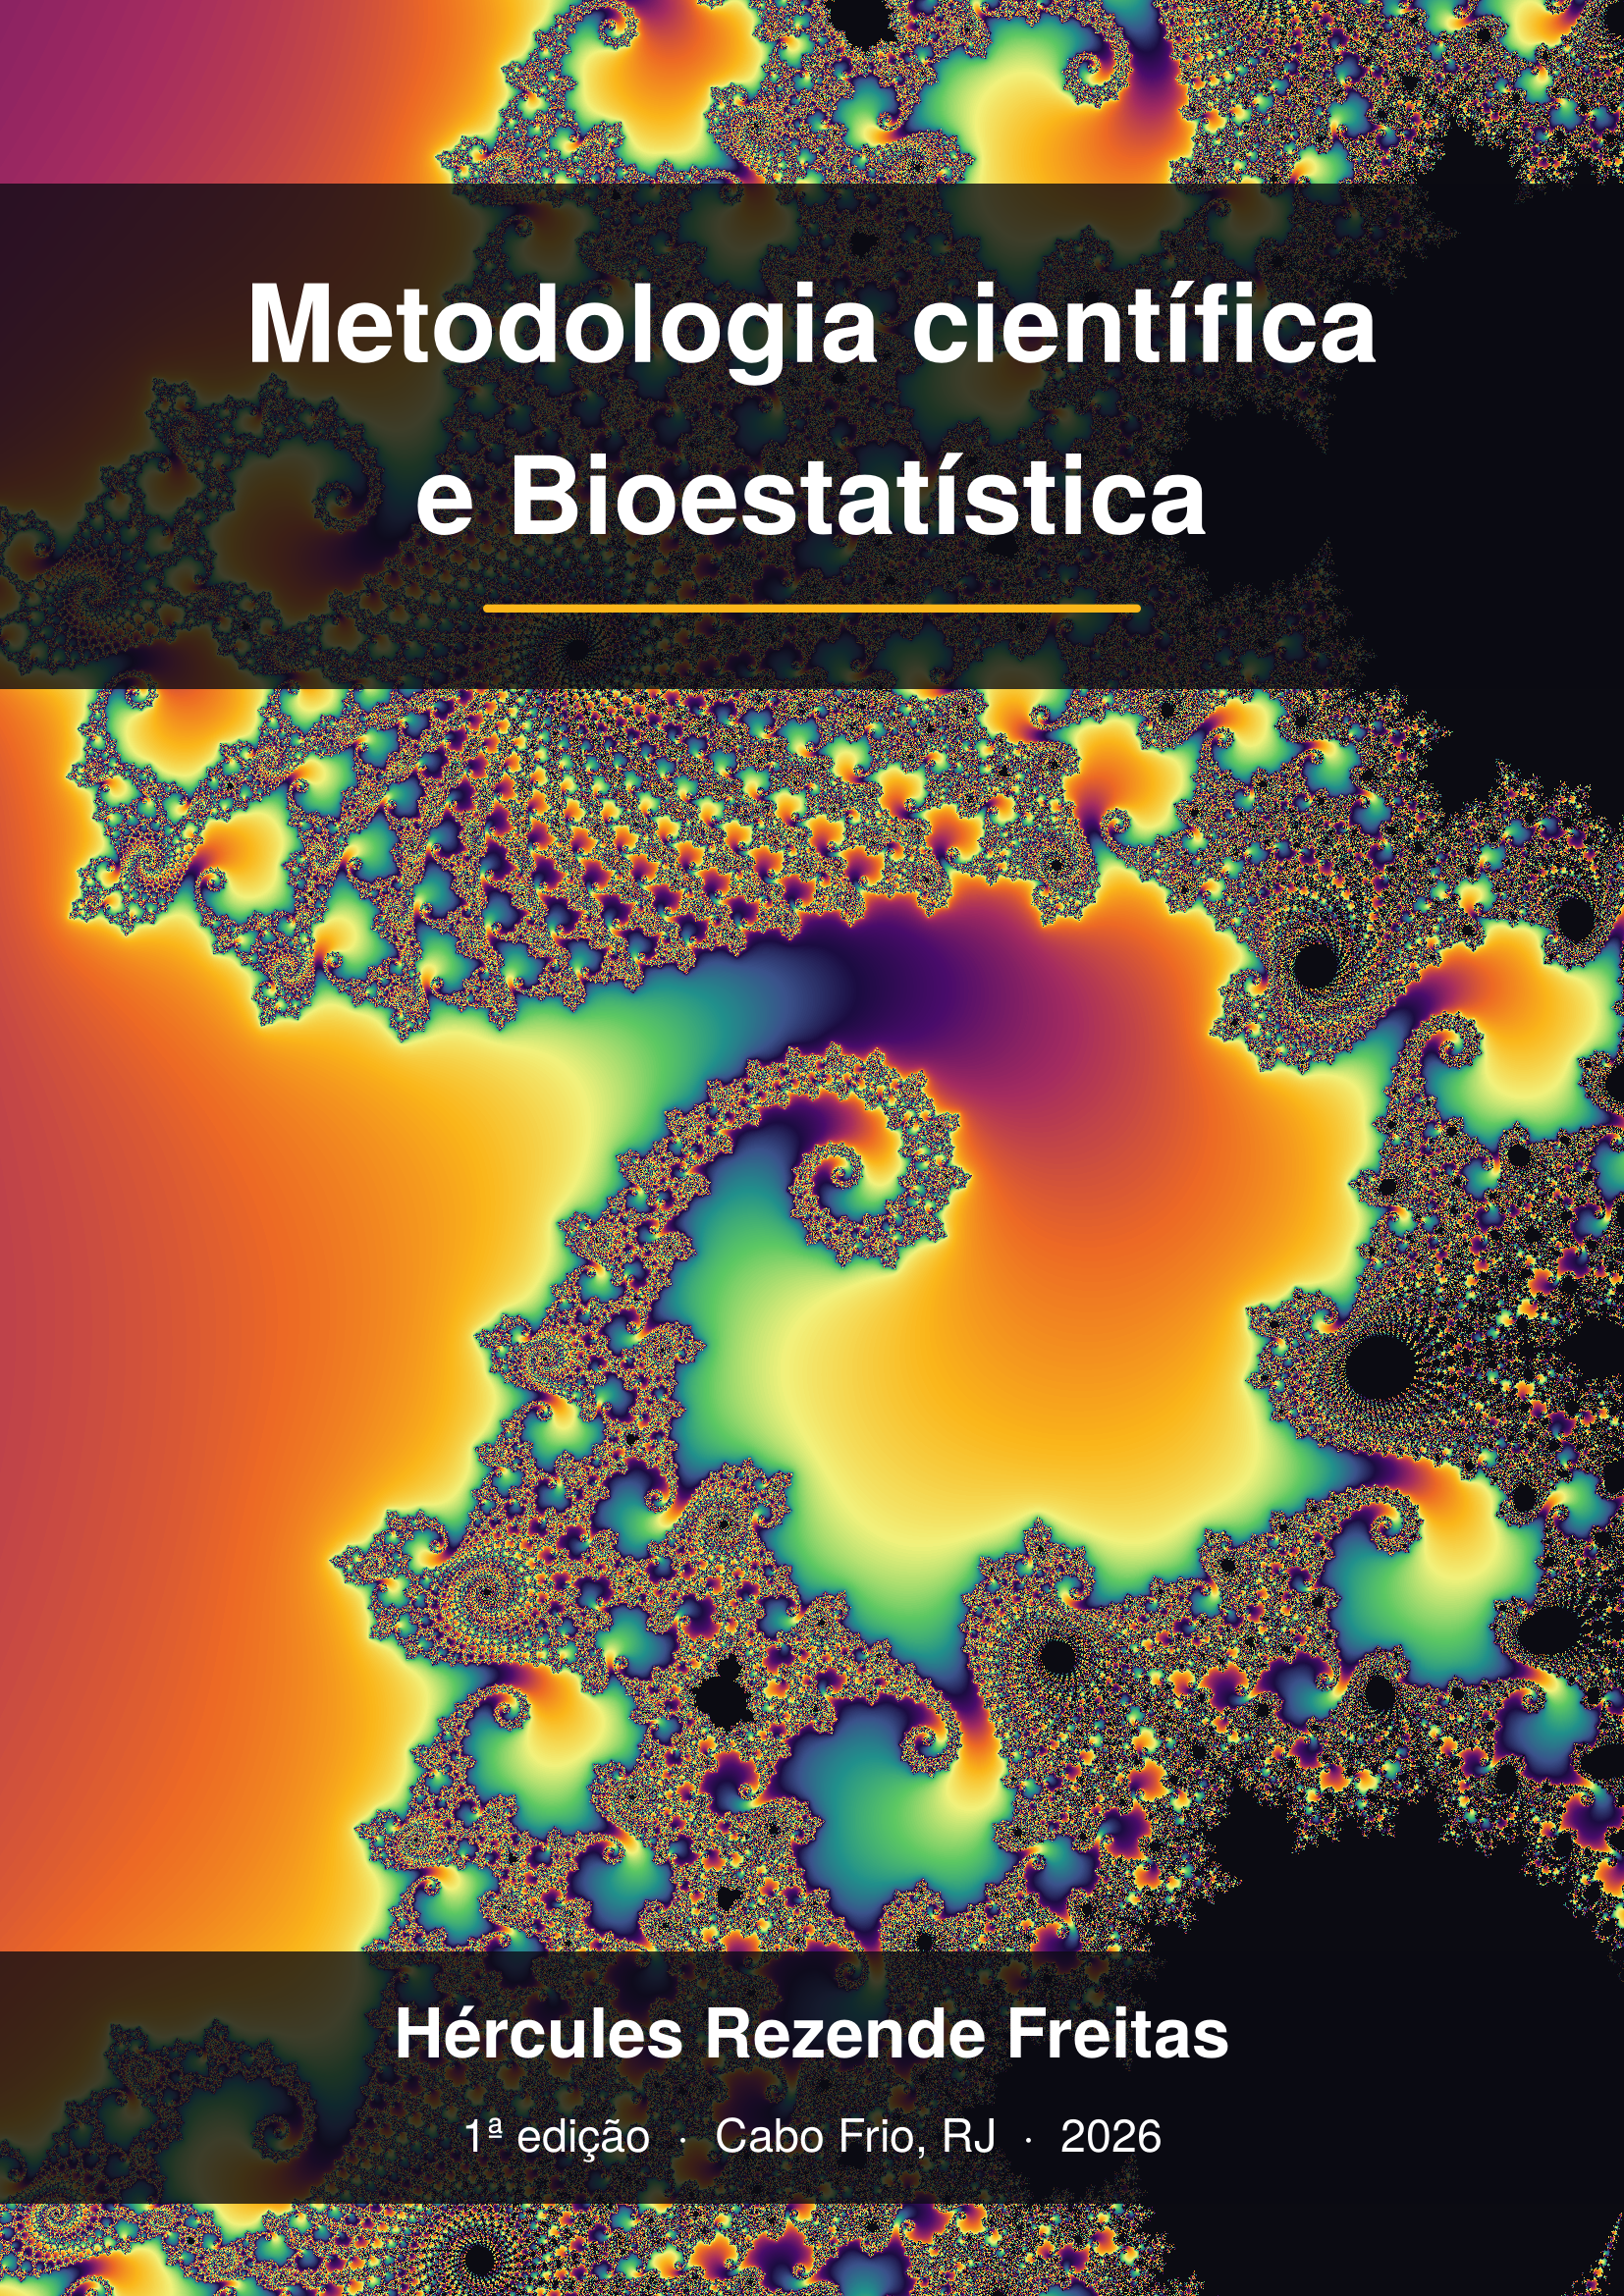
\includegraphics[width=\paperwidth, height=\paperheight]{images/MCBS_capa.png}};
    \end{tikzpicture}
  \end{titlepage}
  \thispagestyle{empty}\null\clearpage
  % Folha de rosto
  \begin{titlepage}
    \centering
    {\Large Hércules Rezende Freitas\par}
    \vspace*{0.22\textheight}
    {\Huge\bfseries Metodologia científica\\[0.4em] e Bioestatística\par}
    \vfill
    {\large 1ª edição\par}
    \vspace{2em}
    {\large Cabo Frio, RJ\\[0.3em] 2026\par}
  \end{titlepage}
  % Verso da folha de rosto
  \thispagestyle{empty}
  \begin{flushleft}
  \small
  \textbf{Autor}: Hércules Rezende Freitas, Universidade do Estado do Rio de Janeiro (UERJ),
  Faculdade de Ciências Médicas, Departamento de Ciências Médicas Integradas, Laboratório de
  Informática em Saúde (LabInfoS), Cabo Frio, RJ, Brasil. ORCID: 0000-0003-1584-9157.
  Contato: hercules.freitas@uerj.br.\par\medskip
  \textbf{Edição}: 1ª edição, Cabo Frio, RJ, 2026. Publicação eletrônica de acesso aberto,
  sem editora (edição do autor).\par\medskip
  \textbf{Texto, revisão, programação, diagramação e capa}: Hércules Rezende Freitas.\par\medskip
  \textbf{Capa}: imagem gerada em R a partir do conjunto de Mandelbrot, com coloração cíclica
  (código em \texttt{capa/capa.R}, no repositório do projeto).\par\medskip
  \textbf{Versão \textit{online}}: \url{https://drhrf.github.io/MCBS/}.
  \textbf{Arquivos-fonte}: \url{https://github.com/drhrf/MCBS}.\par\medskip
  \textbf{Licença}: \textcopyright{} 2026 Hércules Rezende Freitas. Esta obra está licenciada sob a
  licença Creative Commons Atribuição 4.0 Internacional (CC BY 4.0). É permitido copiar,
  redistribuir, adaptar e usar o material para qualquer finalidade, inclusive comercial, desde
  que seja dado o crédito apropriado ao autor, com indicação da fonte, de um link para a licença
  e das alterações realizadas. Texto da licença: \url{https://creativecommons.org/licenses/by/4.0/}.\par\medskip
  \textbf{Declaração sobre o uso de inteligência artificial}: na preparação desta edição, o autor
  utilizou uma ferramenta de inteligência artificial generativa (Claude, da Anthropic) como apoio
  à edição de texto, à escrita e à revisão dos códigos em R e Python. Todo o conteúdo foi revisado
  pelo autor, que é o responsável pelo texto, pelos exemplos, pelos códigos e pelas referências.
  Os exemplos numéricos e os códigos em R são executados a cada compilação do livro, e os
  resultados citados no texto são gerados a partir deles. Por ser uma obra de acesso aberto, em
  permanente aprimoramento, este livro convida leitores, revisores e editores a apontar erros e a
  propor melhorias, conforme descrito na seção \textit{Como contribuir}.\par
  \vfill
  \begin{center}
  \fbox{\parbox{0.8\textwidth}{\centering\vspace{3em}
  Ficha catalográfica\\[0.3em]
  {\footnotesize [a ser inserida após elaboração por bibliotecário]}\\[1em]
  ISBN: [a ser atribuído]\vspace{3em}}}
  \end{center}
  \end{flushleft}
  \clearpage
}
